\documentclass{ximera}

 

\usepackage{epsfig}

\graphicspath{
  {./}
  {figures/}
}

\usepackage{morewrites}
\makeatletter
\newcommand\subfile[1]{%
\renewcommand{\input}[1]{}%
\begingroup\skip@preamble\otherinput{#1}\endgroup\par\vspace{\topsep}
\let\input\otherinput}
\makeatother

\newcommand{\includeexercises}{\directlua{dofile("/home/jim/linearAlgebra/laode/exercises.lua")}}

%\newcounter{ccounter}
%\setcounter{ccounter}{1}
%\newcommand{\Chapter}[1]{\setcounter{chapter}{\arabic{ccounter}}\chapter{#1}\addtocounter{ccounter}{1}}

%\newcommand{\section}[1]{\section{#1}\setcounter{thm}{0}\setcounter{equation}{0}}

%\renewcommand{\theequation}{\arabic{chapter}.\arabic{section}.\arabic{equation}}
%\renewcommand{\thefigure}{\arabic{chapter}.\arabic{figure}}
%\renewcommand{\thetable}{\arabic{chapter}.\arabic{table}}

%\newcommand{\Sec}[2]{\section{#1}\markright{\arabic{ccounter}.\arabic{section}.#2}\setcounter{equation}{0}\setcounter{thm}{0}\setcounter{figure}{0}}

\newcommand{\Sec}[2]{\section{#1}}

\setcounter{secnumdepth}{2}
%\setcounter{secnumdepth}{1} 

%\newcounter{THM}
%\renewcommand{\theTHM}{\arabic{chapter}.\arabic{section}}

\newcommand{\trademark}{{R\!\!\!\!\!\bigcirc}}
%\newtheorem{exercise}{}

\newcommand{\dfield}{{\sf dfield9}}
\newcommand{\pplane}{{\sf pplane9}}

\newcommand{\EXER}{\section*{Exercises}}%\vspace*{0.2in}\hrule\small\setcounter{exercise}{0}}
\newcommand{\CEXER}{}%\vspace{0.08in}\begin{center}Computer Exercises\end{center}}
\newcommand{\TEXER}{} %\vspace{0.08in}\begin{center}Hand Exercises\end{center}}
\newcommand{\AEXER}{} %\vspace{0.08in}\begin{center}Hand Exercises\end{center}}

% BADBAD: \newcommand{\Bbb}{\bf}

\newcommand{\R}{\mbox{$\Bbb{R}$}}
\newcommand{\C}{\mbox{$\Bbb{C}$}}
\newcommand{\Z}{\mbox{$\Bbb{Z}$}}
\newcommand{\N}{\mbox{$\Bbb{N}$}}
\newcommand{\D}{\mbox{{\bf D}}}
\usepackage{amssymb}
%\newcommand{\qed}{\hfill\mbox{\raggedright$\square$} \vspace{1ex}}
%\newcommand{\proof}{\noindent {\bf Proof:} \hspace{0.1in}}

\newcommand{\setmin}{\;\mbox{--}\;}
\newcommand{\Matlab}{{M\small{AT\-LAB}} }
\newcommand{\Matlabp}{{M\small{AT\-LAB}}}
\newcommand{\computer}{\Matlab Instructions}
\newcommand{\half}{\mbox{$\frac{1}{2}$}}
\newcommand{\compose}{\raisebox{.15ex}{\mbox{{\scriptsize$\circ$}}}}
\newcommand{\AND}{\quad\mbox{and}\quad}
\newcommand{\vect}[2]{\left(\begin{array}{c} #1_1 \\ \vdots \\
 #1_{#2}\end{array}\right)}
\newcommand{\mattwo}[4]{\left(\begin{array}{rr} #1 & #2\\ #3
&#4\end{array}\right)}
\newcommand{\mattwoc}[4]{\left(\begin{array}{cc} #1 & #2\\ #3
&#4\end{array}\right)}
\newcommand{\vectwo}[2]{\left(\begin{array}{r} #1 \\ #2\end{array}\right)}
\newcommand{\vectwoc}[2]{\left(\begin{array}{c} #1 \\ #2\end{array}\right)}

\newcommand{\ignore}[1]{}


\newcommand{\inv}{^{-1}}
\newcommand{\CC}{{\cal C}}
\newcommand{\CCone}{\CC^1}
\newcommand{\Span}{{\rm span}}
\newcommand{\rank}{{\rm rank}}
\newcommand{\trace}{{\rm tr}}
\newcommand{\RE}{{\rm Re}}
\newcommand{\IM}{{\rm Im}}
\newcommand{\nulls}{{\rm null\;space}}

\newcommand{\dps}{\displaystyle}
\newcommand{\arraystart}{\renewcommand{\arraystretch}{1.8}}
\newcommand{\arrayfinish}{\renewcommand{\arraystretch}{1.2}}
\newcommand{\Start}[1]{\vspace{0.08in}\noindent {\bf Section~\ref{#1}}}
\newcommand{\exer}[1]{\noindent {\bf \ref{#1}}}
\newcommand{\ans}{}
\newcommand{\matthree}[9]{\left(\begin{array}{rrr} #1 & #2 & #3 \\ #4 & #5 & #6
\\ #7 & #8 & #9\end{array}\right)}
\newcommand{\cvectwo}[2]{\left(\begin{array}{c} #1 \\ #2\end{array}\right)}
\newcommand{\cmatthree}[9]{\left(\begin{array}{ccc} #1 & #2 & #3 \\ #4 & #5 &
#6 \\ #7 & #8 & #9\end{array}\right)}
\newcommand{\vecthree}[3]{\left(\begin{array}{r} #1 \\ #2 \\
#3\end{array}\right)}
\newcommand{\cvecthree}[3]{\left(\begin{array}{c} #1 \\ #2 \\
#3\end{array}\right)}
\newcommand{\cmattwo}[4]{\left(\begin{array}{cc} #1 & #2\\ #3
&#4\end{array}\right)}

\newcommand{\Matrix}[1]{\ensuremath{\left(\begin{array}{rrrrrrrrrrrrrrrrrr} #1 \end{array}\right)}}

\newcommand{\Matrixc}[1]{\ensuremath{\left(\begin{array}{cccccccccccc} #1 \end{array}\right)}}



\renewcommand{\labelenumi}{\theenumi)}
\newenvironment{enumeratea}%
{\begingroup
 \renewcommand{\theenumi}{\alph{enumi}}
 \renewcommand{\labelenumi}{(\theenumi)}
 \begin{enumerate}}
 {\end{enumerate}\endgroup}



\newcounter{help}
\renewcommand{\thehelp}{\thesection.\arabic{equation}}

%\newenvironment{equation*}%
%{\renewcommand\endequation{\eqno (\theequation)* $$}%
%   \begin{equation}}%
%   {\end{equation}\renewcommand\endequation{\eqno \@eqnnum
%$$\global\@ignoretrue}}

%\input{psfig.tex}

\author{Martin Golubitsky and Michael Dellnitz}

%\newenvironment{matlabEquation}%
%{\renewcommand\endequation{\eqno (\theequation*) $$}%
%   \begin{equation}}%
%   {\end{equation}\renewcommand\endequation{\eqno \@eqnnum
% $$\global\@ignoretrue}}

\newcommand{\soln}{\textbf{Solution:} }
\newcommand{\exercap}[1]{\centerline{Figure~\ref{#1}}}
\newcommand{\exercaptwo}[1]{\centerline{Figure~\ref{#1}a\hspace{2.1in}
Figure~\ref{#1}b}}
\newcommand{\exercapthree}[1]{\centerline{Figure~\ref{#1}a\hspace{1.2in}
Figure~\ref{#1}b\hspace{1.2in}Figure~\ref{#1}c}}
\newcommand{\para}{\hspace{0.4in}}

\renewenvironment{solution}{\suppress}{\endsuppress}

\ifxake
\newenvironment{matlabEquation}{\begin{equation}}{\end{equation}}
\else
\newenvironment{matlabEquation}%
{\let\oldtheequation\theequation\renewcommand{\theequation}{\oldtheequation*}\begin{equation}}%
  {\end{equation}\let\theequation\oldtheequation}
\fi

\makeatother


\title{c16.tex}

\begin{document}
\begin{abstract}
BADBAD
\end{abstract}
\maketitle

\chapter{Laplace Transforms}
\label{C:LT}

\normalsize

Laplace transforms are used to solve forced linear differential equations.  
In Section~\ref{sec:2norderinhom} we used the method of undetermined 
coefficients to solve forced equations when the forcing term $g(t)$ is of a 
special form, namely, when $g(t)$ is a linear combination of the functions 
$t^je^{\lambda t}$, $t^je^{\sigma t}\sin(\tau t)$, and 
$t^je^{\sigma t}\cos(\tau t)$.  Although Laplace transforms can be used to 
solve such systems as well, it is usually more efficient to use the method of 
undetermined coefficients when that method is applicable.  The strength of the 
method of Laplace transforms is that it can be used to solve forced linear 
differential equations when the forcing term is more general.  Specifically,
Laplace transforms can be used to solve forced equations when the forcing
term is either discontinuous (a step function) or an impulse function (a Dirac 
delta function).

The idea behind the {\em Laplace transform method} is that it is possible to 
transform any function so that there is a simple relationship between the 
transform of that function and the transform of its derivative.  It is this 
observation, coupled with linearity, that leads to a useful and elegant
method for solving linear, higher order, inhomogeneous differential equations.
In Section~\ref{S:13.1} we discuss this property and the Laplace
transform method for solving differential equations.  In Section~\ref{S:13.3}
we formally introduce the Laplace transform (as an improper integral), show
that this definition satisfies the basic properties introduced in
Section~\ref{S:13.1}, and compute the Laplace transform for a variety of
functions including step functions and Dirac delta functions.

When using the method of Laplace transforms to solve linear differential
equations, it is immediately clear that this method demands the computation of 
partial fraction expansions.  Some of the details of partial fraction
expansions are discussed in Section~\ref{S:PF}.  

In Section~\ref{S:13.4} we solve several linear differential equations with
discontinuous forcing using the methods developed in the first three sections. 
RLC circuits provide an excellent example of a physical problem modeled by
second order linear forced differential equations, and this model is discussed
in Section~\ref{S:SOFE}.  Discontinuous periodic forcing (AC current) also
occurs in these models and their analysis is discussed in that section.


\section{The Method of Laplace Transforms} \label{S:13.1}

In this section we describe the basic properties of Laplace transforms and 
show how these properties lead to a method for solving forced equations.   
We also discuss the kind of information that we will need about Laplace 
transforms in order to solve a general second order forced equation. 

\subsection*{The Basic Properties}

Suppose that there is an operation or transform that transforms functions $x$ 
defined on a variable $t$ to functions ${\cal L}[x]$ defined on a variable 
$s$ in such a way that:
\begin{equation}  \label{Tprops}
\begin{array}{cl}
(a) & {\cal L}\; \mbox{is linear},\\
(b) & {\cal L}\; \mbox{is invertible},\; \mbox{and}\\
(c) & {\cal L}[\dot{x}](s) = s{\cal L}[x](s) - x(0).
\end{array}
\end{equation}\index{Laplace transform!general properties}
Note that \Ref{Tprops}(c) relates the transform of the derivative of a 
function to the transform of the function itself.  We call a transform that 
satisfies \Ref{Tprops} the {\em Laplace transform\/}, as there is only one 
transform that satisfies these three properties.

\subsubsection*{The Laplace Transform of $e^{at}$}

We can use properties \Ref{Tprops} to compute the Laplace transform of the
function $x(t) = e^{at}$.  To perform this calculation we need only recall 
that $e^{at}$ is the unique solution to the differential equation 
$\dot{x}=ax$ with initial value $x(0)=1$.  In essence, we can compute the 
Laplace transform of $e^{at}$ without actually having defined the Laplace 
transform.

It follows from the differential equation $\dot{x}=ax$ and \Ref{Tprops}(a) 
that
\[
{\cal L}[\dot{x}](s) = {\cal L}[ae^{at}](s) = a{\cal L}[e^{at}](s)
\]
and from \Ref{Tprops}(c) that
\[
{\cal L}[\dot{x}](s) = s{\cal L}[e^{at}](s)-1.
\]
Equating these two expressions for ${\cal L}[\dot{x}]$ leads to
\[
s{\cal L}[e^{at}](s)-1 = a{\cal L}[e^{at}](s),
\]
and hence to 
\begin{equation} \label{eq:Lexp}
{\cal L}[e^{at}](s) = \frac{1}{s-a}.
\end{equation}

\subsubsection*{Solving an Inhomogeneous Equation by Laplace Transforms}

Properties \Ref{Tprops} and formula \Ref{eq:Lexp} allow us to solve the 
initial value problem 
\begin{equation} \label{eq:expODE}
\begin{array}{crcl}
(a) & \dot{x} - 3x & = & e^{2t}\\
(b) & x(0) & = & 1.
\end{array}
\end{equation}

Before proceeding, note that \Ref{eq:expODE} can be solved directly using
the method of undetermined coefficients.  \index{undetermined coefficients}  
Indeed, undetermined coefficients show that $x_p(t) = 2e^{2t}$ is a 
particular solution to \Ref{eq:expODE}(a).  Since the general solution to the 
homogeneous equation is $\alpha e^{3t}$, the general solution to the 
inhomogeneous equation \Ref{eq:expODE}(a) is:
\[
x(t) = 2e^{2t} + \alpha e^{3t}.
\]
Setting $\alpha=-1$ solves the initial value problem \Ref{eq:expODE}(b).

We illustrate the method of Laplace transforms by solving \Ref{eq:expODE} 
using Laplace transforms.  Apply the transform ${\cal L}$ to both sides of 
\Ref{eq:expODE}, obtaining 
\[
{\cal L}[\dot{x}-3x](s) = {\cal L}[e^{2t}](s).
\]
From \Ref{eq:Lexp} with $a=2$, we see that
\[
{\cal L}[e^{2t}](s) = \frac{1}{s-2}
\]
Using \Ref{Tprops}(c,a), we see that  
\[
{\cal L}[\dot{x}-3x](s) = (s-3){\cal L}[x](s) - 1.
\]
Hence 
\[
(s-3){\cal L}[x](s) = 1 + \frac{1}{s-2}.
\]

Next, we solve for ${\cal L}[x](s)$, obtaining
\[
{\cal L}[x](s) = \frac{1}{s-3} + \frac{1}{(s-2)(s-3)}.
\]
Using partial fractions\index{partial fractions}, we find  
\[
{\cal L}[x](s)  = \frac{2}{s-3} - \frac{1}{s-2}.
\]
We describe the method of partial fractions in more detail in 
Section~\ref{S:PF}.  The particular uses of partial fractions in this section 
all follow from Exercise~\ref{Ex:pf}. 

Finally, from \Ref{eq:Lexp} we see that 
\[
{\cal L}[2e^{3t}-e^{2t}](s) = \frac{2}{s-3} - \frac{1}{s-2},
\]
and using \Ref{Tprops}(b) we conclude that
\[
x(t) = 2e^{3t}-e^{2t} 
\]
is the unique solution to the initial value problem \Ref{eq:expODE}. 

\subsection*{Three Steps in Solving Equations by Laplace Transforms} 

We can summarize the method for solving ordinary differential equations by
Laplace transforms in three steps.  In this summary it will be useful to 
have defined the inverse Laplace transform.
\begin{Def}  \label{D:invLaplace}
The {\em inverse Laplace transform\/} of a function $Y(s)$ is the function 
$y(t)$ satisfying ${\cal L}[y(t)](s) = Y(s)$, and is denoted by  
${\cal L}\inv[Y(s)]$.
\end{Def}\index{Laplace transform!inverse}

The summary of the Laplace transform method is: 
\begin{enumerate}
\item	Compute the Laplace transforms of both sides of the differential 
equation in \Ref{e:2ndforced} using the linearity of Laplace transforms, the 
formulas for Laplace transforms of derivatives \Ref{Tprops}(c), and specific 
Laplace transforms such as in \Ref{eq:Lexp}.
\item	Explicitly solve the transformed equation for 
${\cal L}[x(t)](s)=Y(s)$.
\item	Find a function $x(t)$ whose Laplace transform is $Y(s)$; that is, 
find ${\cal L}\inv[Y(s)]$.
\end{enumerate}

\subsubsection*{An Example of a First Order Forced Equation}

As an example, we use this three step method to solve the initial value 
problem:
\begin{equation}  \label{eq:dxx2}
\begin{array}{rcl}
\dot x - x & = & 2\\
  x(0) & = & 4.
\end{array}
\end{equation}

The first step is to apply the Laplace transform to both sides of the 
differential equation.  Using formula \Ref{Tprops}(c) and the linearity of 
${\cal L}$, we obtain
\[
\frac{2}{s} = {\cal L}[2] = {\cal L}[\dot x]-{\cal L}[x] = 
(s-1){\cal L}[x]-4.
\]
Note that $e^{0t}=1$ so that ${\cal L}[1] = \frac{1}{s-0}=\frac{1}{s}$.

The second step requires solving this equation explicitly for ${\cal L}[x]$
obtaining
\begin{equation}  \label{eq:Lapdxx2}
{\cal L}[x] = \frac{\frac{2}{s}+4}{s-1} = \frac{2+4s}{s(s-1)}
= \frac{6}{s-1} - \frac{2}{s}.
\end{equation}
Note that we have simplified the right hand side by use of partial fractions.

The third step requires using \Ref{eq:Lexp} to see that
\[
x(t) = {\cal L}\inv\left[\frac{6}{s-1} - \frac{2}{s}\right](t) = 
6{\cal L}\inv\left[\frac{1}{s-1}\right](t) -
2{\cal L}\inv\left[\frac{1}{s}\right](t) = 6e^t-2.
\]


\subsection*{Laplace Transforms of Second Order Equations}

We end this section with a discussion of the type of information that
we will need to solve initial value problems of second order inhomogeneous 
\index{inhomogeneous} linear equations by the method of Laplace transforms. 
Consider the differential equation
\begin{equation}  \label{e:2ndforced}
\begin{array}{rcl} 
\ddot{x} + a\dot{x} + bx & = & g(t)\\
x(0) & = & x_0\\
\dot{x}(0) & = & \dot{x}_0,
\end{array}
\end{equation}
where $a,b\in\R$ are constants.  The function $g(t)$ is called the 
{\em forcing\/} term. 

\subsubsection*{A Second Order Homogeneous Example}
\index{differential equation!higher order}

We begin our discussion by considering a simple example of an unforced 
equation:
\begin{equation}  \label{Lexam2}
\begin{array}{rcl}
\ddot{x} + 3\dot{x} +2x & = & 0  \\
 x(0) & = & 1 \\
\dot{x}(0) & = & 2.
\end{array}
\end{equation}
We begin by applying \Ref{Tprops}(c) twice to obtain
\[
\begin{array}{rcl}
{\cal L}[\ddot{x}](s) & = & s{\cal L}[\dot{x}](s) - \dot{x}(0)\\
& = & s(s{\cal L}[x](s) - x(0)) - \dot{x}(0)\\
& = & s^2{\cal L}[x](s) - sx(0) - \dot{x}(0).
\end{array}
\]
Where there is no ambiguity we will drop the argument $(s)$ in 
${\cal L}[x](s)$; this change should make subsequent formulas easier 
to read.  For instance, the previous equation is:
\begin{equation}  \label{eq:dderLap}
{\cal L}[\ddot{x}] = s^2{\cal L}[x] - sx(0) - \dot{x}(0).
\end{equation}
Now apply \Ref{Tprops} and \Ref{eq:dderLap} to the differential
equation \Ref{Lexam2} to obtain
\begin{eqnarray*}
0 & = & {\cal L}[\ddot{x} + 3\dot{x} +2x] \\
& = & (s^2{\cal L}[x] - sx(0) - \dot{x}(0)) + 
3(s{\cal L}[x] - x(0)) + 2{\cal L}[x]\\
& = & (s^2+3s+2){\cal L}[x] -(sx(0)+\dot{x}(0)+3x(0)) \\
& = & (s^2+3s+2){\cal L}[x] - (s+5).
\end{eqnarray*}

Next, use this equation and partial fractions to solve for ${\cal L}[x]$ as
\[
\dps{\cal L}[x] = \frac{s+5}{(s+1)(s+2)} = 4\frac{1}{s+1} - 3\frac{1}{s+2}.
\]
Using linearity and \Ref{eq:Lexp}, we see that 
\[
{\cal L}[4e^{-t}-3e^{-2t}] = 4\frac{1}{s+1} - 3\frac{1}{s+2}.
\]
Hence
\[
x(t) = 4e^{-t}-3e^{-2t}
\]
is the solution to \Ref{Lexam2}.


\subsubsection*{Information Needed to Solve Second Order Equations}

What information about Laplace transforms will we need to solve the 
initial value problem \Ref{e:2ndforced} in general?  We can answer this 
question just by taking the Laplace transform of \Ref{e:2ndforced} and 
solving for ${\cal L}[x]$.  Using \Ref{eq:dderLap} and \Ref{Tprops}(c), 
compute 
\begin{eqnarray*}
{\cal L}[g(t)] & = & {\cal L}[\ddot{x}+a\dot{x} + bx] \\
& = & {\cal L}[\ddot{x}] + a{\cal L}[\dot{x}]+b {\cal L}[x] \\ 
& = & (s^2{\cal L}[x]-sx_0-\dot{x}_0) +a(s{\cal L}[x]-x_0)+b{\cal L}[x]\\
& = & (s^2+as+b){\cal L}[x]-(x_0s+ax_0+\dot{x}_0).
\end{eqnarray*}
Then solve for ${\cal L}[x]$ as
\begin{equation}  \label{e:laplace2nd}
{\cal L}[x] = \frac{x_0s + ax_0+\dot{x}_0}{s^2+as+b} + \frac{G(s)}{s^2+as+b}
\end{equation}
where $G = {\cal L}[g(t)]$.  The third step in solving \Ref{e:2ndforced}
by Laplace transforms is to compute the inverse Laplace transform
\index{Laplace transform!inverse} of the right hand side of 
\Ref{e:laplace2nd}.  

To find the inverse Laplace transform of the first term, we use partial 
fractions.  For example, suppose that the polynomial $s^2+as+b$ 
has real distinct roots $r_1$ and $r_2$, then we can rewrite the first 
term as 
\[
\frac{c_1}{s-r_1} + \frac{c_2}{s-r_2}
\]
for some real constants $c_1$ and $c_2$.  We can now use \Ref{eq:Lexp}
to find the inverse Laplace transform of this first term.  

If this polynomial has a double real root or a complex conjugate pair of 
roots, then we need to find inverse Laplace transforms of functions like
\begin{equation}  \label{e:sampleLT}
\frac{1}{(s-r_1)^2}  \AND \frac{1}{(s-B)^2+C^2} \AND \frac{s}{(s-B)^2+C^2}.
\end{equation}

Finding the inverse Laplace transform for the second term is in general 
more difficult, since it depends on the hitherto unspecified function $g(t)$.
As it happens this inverse Laplace transform can be computed for a number 
of important functions, as we discuss in the next section.

To summarize: in order to use the method of Laplace transforms successfully
to solve forced second order linear equations, we must be able to
\begin{itemize}
\item	compute partial fraction\index{partial fractions} expansions,
\item	compute the inverse Laplace transforms
\index{Laplace transform!inverse} for functions in \Ref{e:sampleLT}, and
\item   compute the inverse Laplace transforms of the second term in 
\Ref{e:laplace2nd}, which involves the forcing function $g(t)$.
\end{itemize}


\EXER

\TEXER

\begin{exercise} \label{c13.1.0a}
Find the Laplace transform of $x(t)=e^{3t}-2e^{-4t}$.
\end{exercise}

\begin{exercise} \label{c13.1.0b}
Find the Laplace transform of $x(t)=14e^{-6t}+3e^{7t}$.
\end{exercise}

\begin{exercise}  \label{Ex:pf}
Given distinct roots $r_1$ and $r_2$, the method of partial fractions states 
that 
\begin{equation} \label{E:pfquad}
\frac{1}{(s-r_1)(s-r_2)} = \frac{a_1}{s-r_1} + \frac{a_2}{s-r_2}
\end{equation}
for some scalars $a_1$ and $a_2$.  By putting the right side of \Ref{E:pfquad}
over a common denominator, verify that $a_1$ and $a_2$ are found by solving 
the system of linear equations
\begin{eqnarray*}
a_1 + a_2 & = & 0\\
r_2a_1 + r_1a_2 & = & -1.
\end{eqnarray*}
\end{exercise}

\noindent In Exercises \ref{c13.1.0A} -- \ref{c13.1.0B} use partial fractions
to find a function $x(t)$ whose Laplace transform is the given function
$Y(s)$.  {\bf Hint:}  In your calculations, you may use the result of 
Exercise~\ref{Ex:pf}.
\begin{exercise} \label{c13.1.0A}
$Y(s) = \dps\frac{1}{s^2-4s+3}$.
\end{exercise}
\begin{exercise} \label{c13.1.0B}
$Y(s) = \dps\frac{s-1}{s^2+5s+6}$.
\end{exercise}


\noindent In Exercises~\ref{c13.1.1} -- \ref{c13.1.1a}, use Laplace transforms 
to compute the solution to the given initial value problem.
\begin{exercise} \label{c13.1.1}
$\ddot{x} + 3\dot{x} + 2x = 0, \quad x(0) = 1, \quad \dot{x}(0) = -1$. 
\end{exercise}
\begin{exercise} \label{c13.1.1a}
$\ddot{x} - 3\dot{x} - 4x = 0, \quad x(0) = 2, \quad \dot{x}(0) = -1$. 
\end{exercise}

\begin{exercise} \label{c13.4.4}
Let $\alpha,\beta,a,b,c$ be real numbers.  Show that the solution
of the initial value problem
\[
\ddot x +a\dot x +b x=c,\quad x(0)=\alpha,\quad \dot x(0)=\beta,
\]
has the Laplace transform
\[
{\cal L}[x] = \frac{\alpha s^2 +(\beta +a\alpha)s+c}{s(s^2+as+b)}.
\]
\end{exercise}

\begin{exercise}   \label{exer:kderLap}
Identity \Ref{eq:dderLap}\index{Laplace transform!derivative property} may be 
generalized to: 
\begin{equation}  \label{LapDerk}
{\cal L}\left[\frac{d^k y}{dt^k}\right] =
s^k{\cal L}[y] - s^{k-1} y(0) - \cdots - \frac{d^{k-1} y}{dt^{k-1}}(0).
\end{equation}
Use induction to verify \Ref{LapDerk}. 
\end{exercise}


\section{Laplace Transforms and Their Computation} \label{S:13.3}
\index{Laplace transform!existence}

This section divides into three parts.  In the first part, we give an explicit 
formula for the Laplace transform and verify that this formula satisfies 
properties \Ref{Tprops}.  In the second part, we compute a table of Laplace
transforms for a number of special functions including step functions and
impulse functions.  In the third part we discuss two properties of Laplace
transforms that are useful when computing inverse Laplace transforms of
functions of the type that appear when solving forced second order equations.

\begin{Def}  \label{D:laplace}
Let $x(t)$ be a function that is defined for $0\le t < \infty$.
Then the function ${\cal L}[x](s)$ is defined by
\begin{equation} \label{E:laplace}
{\cal L}[x](s) = \int_0^{\infty} e^{-st} x(t)\; dt
\end{equation}
and is called the {\em Laplace transform\/} of $x(t)$.
\end{Def}\index{Laplace transform!definition}

Note that the Laplace transform is an improper 
integral --- which implies that some care must be taken when discussing 
its properties.  Indeed, for some functions the Laplace transform does 
not exist for all values of $s$.  What usually happens is that 
the Laplace transform exists for all values of $s$ larger than some 
number $a$.  As an example, we compute \Ref{eq:Lexp} directly using 
Definition~\ref{D:laplace}.  Let $x(t)=e^{at}$ and compute 
\begin{equation}  \label{e:expat}
{\cal L}[x](s) = \int_0^{\infty} e^{(a-s)t}\; dt=
\lim\limits_{h\to \infty} \frac{1}{s-a}\left( 1-e^{(a-s)h} \right)
=\left\{ \begin{array}{cl} \frac{\dps 1}{\dps s-a} & \mbox{for $s>a$,}\\
\infty & \mbox{for $s\le a$.}\end{array}\right.
\end{equation}

\subsubsection*{The Laplace Transform is Linear}
\index{Laplace transform!linearity}

The first step in verifying properties \Ref{Tprops} is to show that the 
Laplace transform ${\cal L}$ is linear, that is, to 
show that \Ref{Tprops}(a) holds.
\begin{prop}  \label{prop:linLap}
Suppose $x(t)$ and $y(t)$ are functions for which the Laplace transforms
${\cal L}[x](s)$, ${\cal L}[y](s)$ exist for $s>a$, and let $c$ be real. 
Then for all $s>a$
\begin{equation}  \label{eq:linLap}
\begin{array}{rcl}
{\cal L}[x + y] &  = & {\cal L}[x] + {\cal L}[y] \\
{\cal L}[cx] & = & c{\cal L}[x].
\end{array}
\end{equation}
\end{prop}

\begin{proof} Using properties of integrals we obtain for each $s>a$
\begin{eqnarray*}
{\cal L}[x+y](s) &=& \int_0^{\infty} e^{-st} (x(t)+y(t))\; dt\\
&=& \int_0^{\infty} e^{-st} x(t)\; dt + \int_0^{\infty} e^{-st} y(t)\; dt\\
&=& {\cal L}[x](s)+ {\cal L}[y](s).
\end{eqnarray*}
A similar computation verifies that ${\cal L}$ commutes with scalar 
multiplication.  \end{proof}

\subsubsection*{The Derivative Property of Laplace Transforms is Valid}
\index{Laplace transform!derivative property}

Next we verify the important derivative property \Ref{Tprops}(c) of the 
Laplace transform.  

\begin{prop}  \label{prop:derLap}
Suppose that $x$ is a differentiable function such that 
$|x(t)|\le Me^{at}$ for constants $a>0$ and $M>0$.  
Then
\begin{itemize}
\item[(a)] the Laplace transform ${\cal L}[x](s)$ exists for $s>a$; 
\item[(b)] ${\cal L}[\dot x](s) = s{\cal L}[x](s) - x(0) \quad 
\mbox{for $s>a$.}$
\end{itemize}
\end{prop}

\begin{proof} 
\noindent (a) Observe that by the assumption on the growth of 
$x(t)$ we have for $s>a$
\[
\lim\limits_{h\to \infty}\left|\int_0^h e^{-st} x(t)\; dt\right|
\le \lim\limits_{h\to \infty}\int_0^h Me^{(a-s)t}\; dt
=\lim\limits_{h\to \infty}\left.\frac{Me^{(a-s)t}}{a-s}\right|_0^h
=\frac{M}{s-a}<\infty.
\]
Hence the Laplace transform ${\cal L}[x](s)$ exists for $s>a$.

\noindent(b) First note that
\[
\lim\limits_{h\to \infty} |e^{-sh} x(h)|\le
\lim\limits_{h\to \infty} |Me^{(a-s)h}| = 0.
\]
Now use the definition of improper integrals and integration by parts to 
compute 
\begin{eqnarray*}
{\cal L}[\dot x](s) &=& \int_0^{\infty} e^{-st} \dot x(t)\; dt\\
& = & \lim\limits_{h\to \infty}\int_0^h e^{-st} \dot x(t)\; dt\\
& = & \lim\limits_{h\to \infty}\left(\left.e^{-st}x(t)\right|_0^h -
\int_0^h (-s)e^{-st} x(t)\; dt\right)\\
&=& \lim\limits_{h\to \infty} \left( e^{-sh} x(h) - x(0)\right) +
s\lim\limits_{h\to \infty} \int_0^h e^{-st} x(t)\; dt\\
&=& -x(0) + s{\cal L}[x](s)
\end{eqnarray*}
for $s>a$.  \end{proof}

Finally, we remark that \Ref{Tprops}(b) is valid, but that its proof is 
beyond the scope of this course.  One method of proof is to develop an 
explicit integral formula for the inverse Laplace transform. 


\subsection*{A Table of Laplace Transforms}
\index{Laplace transform!table of}

In order to solve differential equations using the method of Laplace 
transforms, we need to have a table of Laplace transforms readily available.  
We now compute the Laplace transform for the functions in 
Table~\ref{tab:Laplist}.   These functions include the discontinuous step 
function\index{step function} 
\[
H_c(t) = \left\{\begin{array}{ll}
0 & \mbox{for $0\le t < c$}\\
1 & \mbox{for $t\ge c$}
\end{array}\right. 
\]\index{$H_c(t)$}
where $c$ is a positive constant and the hitherto undefined Dirac delta 
function $\delta_c(t)$.  See Figure~\ref{F:H1} for a graph of $H_1$.

\begin{figure}[htb]
           \centerline{%
           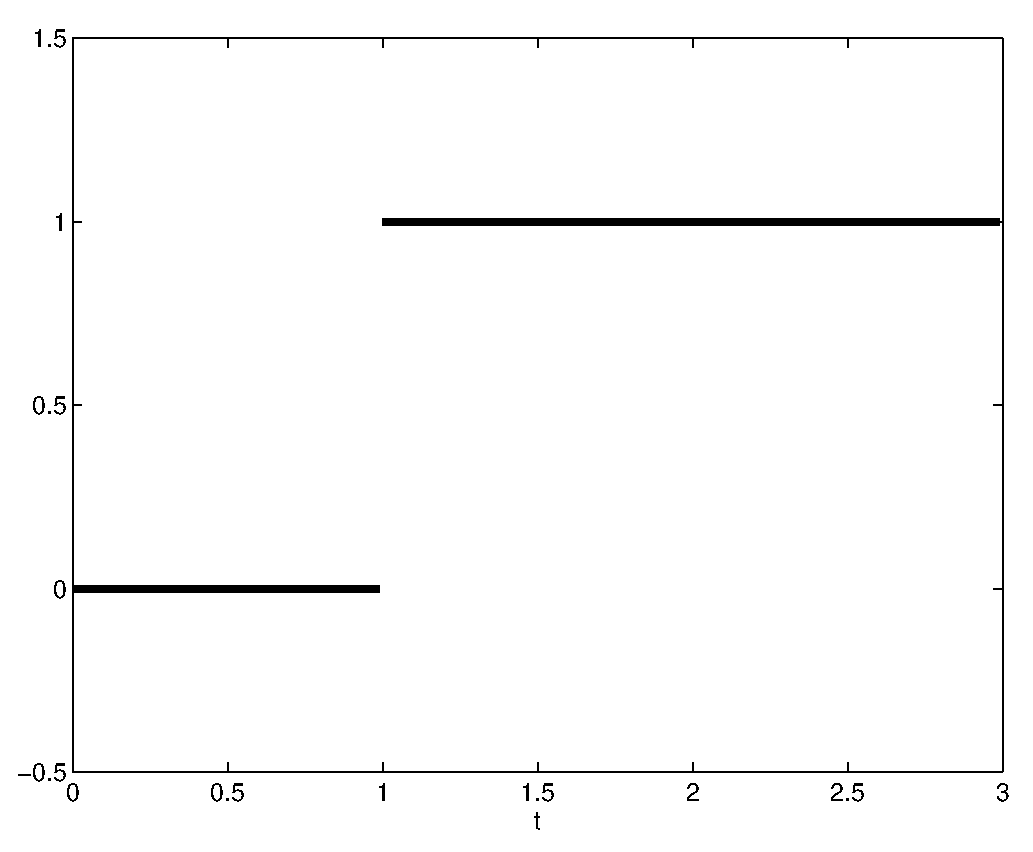
\psfig{file=figures/H1.eps,width=2.5in}}
           \caption{Graph of $H_1(t)$.}
           \label{F:H1}
\end{figure}

We derive some of these formulas by using the Laplace transform formulas for 
derivatives \Ref{Tprops}(c) and \Ref{eq:dderLap}.  (We could compute these 
transforms directly by integration from Definition~\ref{D:laplace}, but the 
method we choose is simpler and illustrates the power of the derivative 
formulas.)  Note that we have already computed the Laplace transforms 
of the first two functions in Table~\ref{tab:Laplist} when deriving 
\Ref{eq:Lexp}.

\begin{table}[htb]
\begin{center}
\begin{tabular}{|c|c|}
\hline
Function $y(t)$ & Laplace transform ${\cal L}[y](s)$\\
\hline
$1$ & $\frac{\dps 1}{\dps s}$\\
$e^{at}$ & $\frac{\dps 1}{\dps s-a}$\\
$\cos(\tau t)$ & $\frac{\dps s}{\dps s^2 + \tau^2}$\\
$\sin(\tau t)$ & $\frac{\dps \tau}{\dps s^2 + \tau^2}$\\
$t^n$ & $\frac{\dps n!}{\dps s^{n+1}}$\\
$H_c(t)$ & $\frac{1}{\dps s}e^{-cs}$\\
$\delta_c(t)$ & $e^{-cs}$\\
\hline
\end{tabular}
\end{center}
\caption{Laplace transforms.}
\label{tab:Laplist}
\end{table}


\subsubsection*{The Laplace Transforms: ${\cal L}[\cos(\tau t)]$ and 
${\cal L}[\sin(\tau t)]$}

To compute ${\cal L}[x]$ where $x(t)=\cos(\tau t)$, observe that $x(t)$ is 
a solution to the initial value problem
\begin{eqnarray*}
\ddot{x}+\tau^2 x & = & 0\\ 
x(0) & = & 1 \\ 
\dot{x}(0) & = & 0.
\end{eqnarray*}
It follows from \Ref{eq:dderLap} that
\[
s^2{\cal L}[x] - s + \tau^2 {\cal L}[x] = 0.
\]
Hence
\[
{\cal L}[x] = \frac{s}{s^2+\tau^2},
\]
as desired.  Similarly, note that $x(t)=\sin(\tau t)$ satisfies the initial
value problem
\begin{eqnarray*}
\ddot{x}+\tau^2 x & = & 0 \\
  x(0) & = & 0 \\
 \dot{x}(0) & = & \tau.
\end{eqnarray*}
The computation of the Laplace transform for $\sin(\tau t)$ proceeds
identically as the computation of ${\cal L}[\cos(\tau t)]$.

\subsubsection*{The Laplace Transform: ${\cal L}[t^n]$}

Next, we compute ${\cal L}[t^n]$ by applying \Ref{Tprops}(c) $n$ times.
That is, 
\[
{\cal L}[t^n] = \frac{n}{s}{\cal L}[t^{n-1}] = \cdots =
\frac{n!}{s^n}{\cal L}[1] = \frac{n!}{s^{n+1}}.
\]

\subsubsection*{The Laplace Transform: ${\cal L}[H_c(t)]$}

We compute the Laplace transform of the step function $H_c(t)$ by direct 
integration.  
\[
{\cal L}[H_c](s) = \int_0^{\infty} e^{-st}H_c(t)\; dt
= \int_c^{\infty} e^{-st}\; dt
=\left\{ \begin{array}{cl} \frac{1}{\dps s}e^{-cs} & \mbox{for $s>0$,}\\
\infty & \mbox{for $s\le 0$.}\end{array}\right.
\]


\subsubsection*{The Laplace Transform of Dirac Delta Functions}
\index{Dirac delta function}

Suppose that a strong external force is applied at time $t=c$, but only for a 
very short time $h$.  Then the forcing function is approximated by
\begin{equation}  \label{eq:deltah}
\begin{array}{rcl}
g_h(t) & =  & 
\left\{\begin{array}{cc} \frac{1}{h} & c\leq t \leq c+h \\ 
		0 & \mbox{otherwise} \end{array} \right. \\
 & = & \frac{1}{h} \left(H_c(t)-H_{c+h}(t)\right). 
\end{array}
\end{equation}
The graph of $g_h$ is given in Figure~\ref{fig:deltah}.  It is not clear how 
to take the limit of $g_h(t)$ as $h\to 0$ in \Ref{eq:deltah}, since this limit 
leads to a `function' that is infinity at $c$ and zero elsewhere.  Despite 
this difficulty, the limit is called the {\em Dirac delta function}
\index{Dirac delta function} and is denoted by $\delta_c(t)$.  We compute the 
Laplace transform of the $\delta_c(t)$ by first computing the Laplace 
transform of the approximating function $g_h(t)$ and then taking the limit of 
the Laplace transforms of the approximation as $h\to 0$.

\begin{figure}[htb]
           \centerline{%
           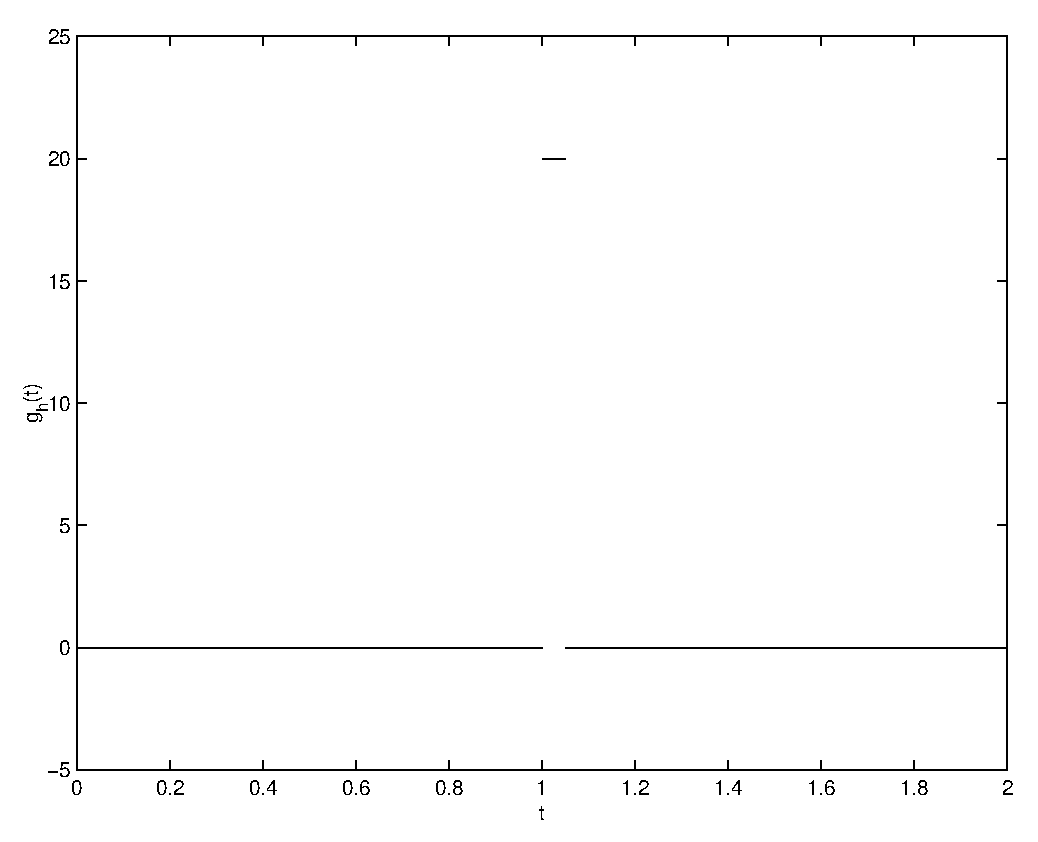
\psfig{file=figures/deltah.eps,width=2.8in}}
           \caption{Graph of the approximating function $g_h(t)$ of  
	   \protect\Ref{eq:deltah} for $c=1$ and $h=0.05$.}
           \label{fig:deltah}
\end{figure}

The Laplace transform of the approximating function $g_h(t)$ is found using 
the linearity of ${\cal L}$ and Table~\ref{tab:Laplist}, that is,
\[
{\cal L}[g_h] =  \frac{1}{h} \left({\cal L}[H_c]-{\cal L}[H_{c+h}]\right) =
\frac{1}{h}\left(\frac{1}{s}e^{-cs}-
\frac{1}{s}e^{-(c+h)s}\right) = \frac{1}{s}e^{-cs}\frac{1-e^{-sh}}{h}.
\]
We claim that
\[
\lim_{h\to 0} \left(\frac{1-e^{-sh}}{h}\right)=s,
\]
from which it follows that 
\[
\lim_{h\to 0} {\cal L}[g_h](s)=e^{-cs}.
\]
This result justifies writing
\begin{equation}  \label{e:lapdel}
{\cal L}[\delta_c] = e^{-cs}.
\end{equation}
To verify the claim, let $f(y)=e^{-sy}$ and recall that 
\[
f'(0) = \lim_{h\to 0} \frac{f(h)-f(0)}{h} =\lim_{h\to 0} \frac{e^{-sh}-1}{h}.
\]
Since $f'(0)=-s$, it follows that
\[
\lim_{h\to 0} \left(\frac{1-e^{-sh}}{h}\right)=-f'(0)=s,
\]
as claimed.


\subsection*{Additional Techniques for Laplace Transforms}

At the end of Section~\ref{S:13.1} we showed that when solving second order
differential equations by the method of Laplace transforms, it is necessary to 
compute inverse Laplace transforms of functions like
\begin{equation}  \label{E:1sttype}
\frac{1}{(s-B)^2+C^2} \AND \frac{s-B}{(s-B)^2+C^2}
\end{equation}
and 
\begin{equation}  \label{2ndtype}
\frac{1}{(s-B)^2+C^2}G(s) \AND \frac{s-B}{(s-B)^2+C^2}G(s)
\end{equation}
where $G(s)$ is the Laplace transform of the forcing function $g(t)$.
See \Ref{e:sampleLT}.  

\subsubsection*{Inverse Laplace Transforms of Shifted Functions}

The next proposition enables us to calculate inverse Laplace transforms for
functions of type \Ref{E:1sttype}.

\begin{prop}  \label{prop:eHcLap1}
Suppose that $Y(s)={\cal L}[y(t)](s)$ exists.  Then
\[
\begin{array}{rrcl}
\mbox{(a)} & {\cal L}[e^{at}y(t)](s) & = & Y(s-a)\\
\mbox{(b)} & {\cal L}^{-1}[Y(s-a)](t) & = & e^{at}y(t).
\end{array}
\]
\end{prop}
\index{Laplace transform!general properties}\index{Laplace transform!inverse}

\begin{proof}  To verify (a) compute
\[
{\cal L}[e^{at}y(t)](s) = \int_0^{\infty} e^{-st}e^{at} y(t)\; dt
= \int_0^{\infty} e^{-(s-a)t} y(t)\; dt = {\cal L}[y(t)](s-a) = Y(s-a).
\]
Part (b) follows by applying the inverse Laplace transform to both sides 
of (a).  \end{proof}

For example, suppose that we want to compute the inverse Laplace transform of 
\begin{equation}  \label{e:exlappf}
\frac{s-1}{s^2+2s+5}.
\end{equation}
The first step in this computation is to write the denominator as the sum of 
two squares and to shift the numerator.   That is,
\begin{equation}  \label{e:pf1}
\frac{s-1}{s^2+2s+5} = \frac{(s+1)-2}{(s+1)^2+4} = 
\frac{s+1}{(s+1)^2+4} - 2\frac{1}{(s+1)^2+4}.
\end{equation}
We can now find the inverse Laplace transform of the right hand side of 
\Ref{e:pf1}.  Except for the shift of $s$ to $s+1$, the rearranged expression 
\Ref{e:pf1} is one whose inverse Laplace transform can be read from 
Table~\ref{tab:Laplist}.  More precisely, let 
\[
Y(s) = \frac{s}{s^2+4} - 2\frac{1}{s^2+4},
\]
so that the right hand side of \Ref{e:pf1} is $Y(s+1)$.  Using 
Table~\ref{tab:Laplist} the inverse Laplace transform of $Y(s)$ is
\begin{equation}  \label{e:exlappf2}
{\cal L}\inv[Y(s)](t) = 
{\cal L}\inv\left[\frac{s}{s^2+4} - 2\frac{1}{s^2+4}\right](t) = 
\cos(2t) - \sin(2t) = y(t).
\end{equation}
Using Proposition~\ref{prop:eHcLap1}(b) we can compute the inverse Laplace 
transform of $Y(s+1)$ 
as
\[
{\cal L}^{-1}[Y(s+1)](t) = e^{-t}y(t)
\]
That is,
\[
{\cal L}^{-1}\left[\frac{s-1}{s^2+2s+5}\right](t) = e^{-t}(\cos(2t)-\sin(2t)).
\]

\subsubsection*{Another Useful Property of the Laplace Transform}

Next, we examine the Laplace transform of a function that is multiplied 
by the jump function $H_c(t)$ and by doing so we will be able to compute the
inverse Laplace transform of functions like \Ref{2ndtype} when $G(s)$ is the 
Laplace transform of a discontinuous forcing function.

\begin{prop}  \label{prop:eHcLap2}
Suppose that $Y(s)={\cal L}[y(t)](s)$ exists.  Then
\[
\begin{array}{rrcl}
\mbox{(a)} & {\cal L}[H_c(t)y(t-c)](s) & = & e^{-cs} Y(s) \\
\mbox{(b)} & {\cal L}^{-1}[e^{-cs}Y(s)](t) & = & H_c(t)y(t-c).
\end{array}
\]
\end{prop}

\begin{proof} (a)  Compute
\[
{\cal L}[H_c(t)y(t-c)](s) = \int_0^{\infty} e^{-st}H_c(t) y(t-c)\; dt
= \int_c^{\infty} e^{-st}y(t-c)\; dt.
\]
On substituting $t+c$ for $t$ we obtain
\[
{\cal L}[H_c(t)y(t-c)](s)=\int_0^{\infty} e^{-s(t+c)}y(t)\; dt
=e^{-cs} \int_0^{\infty} e^{-st}y(t)\; dt
=e^{-cs} Y(s).
\]
Part (b) follows by applying the inverse Laplace transform to both sides 
of (a).  \end{proof}

As an application of Proposition~\ref{prop:eHcLap2}(b), we find that
\[
{\cal L}^{-1}\left[ e^{-s}\frac{s}{s^2+4}\right](t)=
H_1(t){\cal L}^{-1}\left[ \frac{s}{s^2+4}\right](t-1)=
H_1(t)\cos(2(t-1)).
\]

\EXER

\TEXER

\noindent In Exercises~\ref{c13.3.1a} -- \ref{c13.3.1d} compute the Laplace 
transform for each function $x(t)$:
\begin{exercise} \label{c13.3.1a}
$x(t) = 4\cos(t-1)$,
\end{exercise}
\begin{exercise} \label{c13.3.1b}
$x(t) = \sin(3(t-2))$,
\end{exercise}
\begin{exercise} \label{c13.3.1c}
$x(t) = (t-3)^2$.
\end{exercise}
\begin{exercise} \label{c13.3.1d}
$x(t) = te^{-2t}$.
\end{exercise}


\noindent In Exercises~\ref{c13.3.2} -- \ref{c13.2.2}, use Laplace transforms 
to compute the solution to the given initial value problem.
\begin{exercise} \label{c13.3.2}
$\ddot{x} + 2\dot x +5x = 0, \quad x(0) = 2, \quad \dot{x}(0) = -6$.
\end{exercise}
\begin{exercise} \label{c13.4.3a}
$\ddot x +4\dot x +20 x=0,\quad x(0)=1,\quad \dot{x}(0)=-6$.
\end{exercise}
\begin{exercise} \label{c13.4.3b}
$\ddot x -6\dot x +13 x=1,\quad x(0)=0,\quad \dot{x}(0)=1$.
\end{exercise}
\begin{exercise} \label{c13.2.1}
$\ddot{x} + 2\dot{x} - 3x  =  1, \quad x(0) = 2, \quad \dot{x}(0) = 0$.
\end{exercise}
\begin{exercise} \label{c13.2.2}
$\ddot{x} + 2\dot{x} - 8x = e^t, \quad x(0) = 1, \quad \dot{x}(0) = 2$.
\end{exercise}

\begin{exercise} \label{c13.1.2}
Suppose that $z(t)=ty(t)$.  Using \Ref{E:laplace} show that
\[
{\cal L}[z](s) = -\frac{\dps d}{\dps ds} {\cal L}[y](s).
\]
\end{exercise}


\section{Partial Fractions}  \label{S:PF}
\index{partial fractions}

In Section~\ref{S:13.1} we saw that expansions into partial fractions is a 
necessary tool when applying the method of Laplace transforms.  In the
simplest case partial fractions work as follows.  Assume that $p(s)$ and 
$q(s)$ are two polynomials such that
\begin{enumerate}
\item[(a)] the degree of $p(s)$ is less or equal to the degree $d$ of $q(s)$;
\item[(b)] $q(s)=(s-r_1)\cdots(s-r_d)$ has no multiple roots.
\end{enumerate}
The roots $r_1,\ldots,r_d$ of $q(s)$ may be either real or complex.  Then the 
expansion into partial fractions of $p(s)/q(s)$ has the form
\begin{equation}  \label{E:PF}
\frac{p(s)}{q(s)} = \frac{c_1}{s-r_1}+\frac{c_2}{s-r_2}+\cdots
+\frac{c_d}{s-r_d},
\end{equation}
where $c_1,\ldots,c_d$ are  scalars determined from $p$ and $q$.

There is a simple way to compute the constant $c_j$. Define the degree $d-1$
polynomial
\[
q_j(s) = \frac{q(s)}{s-r_j} = 
(s-r_1)\cdots(s-r_{j-1})(s-r_{j+1})\cdots(s-r_d).
\]
Multiply both sides of \Ref{E:PF} by $s-r_j$ and evaluate at $s=r_j$ to 
obtain
\[
c_j = \frac{p(r_j)}{q_j(r_j)}.
\]   

For example, compute the partial fraction expansion for
\[
\frac{s^2+3s-5}{s(s-1)(s+2)} = \frac{c_1}{s}+\frac{c_2}{s-1}+\frac{c_3}{s+2}.
\]
In this example, $r_1=0$, $r_2=1$, and $r_3=-2$.  The relevant polynomials
are:
\[
p(s) = s^2+3s-5 \qquad q_1(s) = (s-1)(s+2) \qquad q_2(s) = s(s+2) \qquad
q_3(s) = s(s-1).
\]
It follows that 
\[
c_1 = \frac{p(0)}{q_1(0)} = \frac{5}{2} \qquad
c_2 = \frac{p(1)}{q_2(1)} = -\frac{1}{3} \qquad
c_3 = \frac{p(-2)}{q_3(-2)} = -\frac{7}{6}.
\]

\subsubsection*{Partial Fractions with Complex Roots}
\index{partial fractions!complex roots}


Suppose that the denominator $q(s)$ has complex conjugate roots $r$ and 
$\overline{r}$.  When $r$ is a complex simple root of $q(s)$, then the 
partial fractions expansion of $p(s)/q(s)$ contains the two terms
\[
\frac{c}{s-r} + \frac{d}{s-\overline{r}}
\]
where $c,d\in\C$.  Together these two terms must be real-valued, and it 
follows that $d=\overline{c}$.  Therefore the expansion is 
\[
\frac{c}{s-r} + \frac{\overline{c}}{s-\overline{r}}
\]
for some complex scalar $c$.  These terms combine as
\[
\frac{c(s-\overline{r})+ \overline{c}(s-r)}{s^2-2r_1s+r\overline{r}}
\]
where $r=r_1+ir_2$.  With inverse Laplace transforms in mind, we prefer 
to write this expression as
\begin{equation}  \label{e:pfreal}
\frac{2c_1(s-r_1)-2c_2r_2}{(s-r_1)^2+r_2^2}
\end{equation}
where $c=c_1+ic_2$.  

In the third part of Section~\ref{S:13.3} we saw how to compute inverse 
Laplace transforms of functions like those in \Ref{e:pfreal}.



\subsection*{Partial Fractions Using \Matlab}
\index{partial fractions!in \Matlab}

The \Matlab command {\tt residue}\index{\computer!residue} can be used to 
determine partial fractions
expansions.  We begin by discussing how polynomials are defined in \Matlabp.  
The polynomial $q(s)=a_ds^d+\cdots+a_1s+a_0$ is stored in \Matlab by the 
vector {\tt q = [ad $\cdots$ a1 a0]} consisting of the coefficients of $q(s)$ 
in {\em descending\/} order.  For instance, in \Matlabp, the polynomial 
$q(s)=2s^3 - 3s +5$ is identified with the vector $(2,0,-3,5)$.  

Suppose that the two vectors {\tt p} and {\tt q} represent the two polynomials 
$p(s)$ (of degree less than $D$) and $q(s)$ (of degree $d$).  Both the vector 
of roots $r=(r_1,\ldots,r_d)$ and the vectors of scalars $c=(c_1,\ldots,c_d)$ 
are determined using the command 
\begin{verbatim}
[c,r] = residue(p,q)
\end{verbatim}

To illustrate this command, find the partial fraction expansion of 
\[
\frac{4s+2}{s^2-s}
\]
(which we computed previously in \Ref{eq:Lapdxx2}) by typing
\begin{verbatim}
    p = [4 2];
    q = [1 -1 0];
[c,r] = residue(p,q)
\end{verbatim}
\Matlab responds with
\begin{verbatim}
c =
     6
    -2
r =
     1
     0
\end{verbatim}
Note that this result agrees with our previous calculation in \Ref{eq:Lapdxx2}.

Observe that the situation where the polynomial $q(s)$ has complex roots 
is not excluded.  Indeed, let $p(s) = s+1$ and $q(s) = s^3+s^2-4s+6$, and type
\begin{verbatim}
    p = [1 1];
    q = [1 1 -4 6];
[c,r] = residue(p,q)
\end{verbatim}
to obtain the answer
\begin{verbatim}
c =
  -0.1176          
   0.0588 - 0.2647i
   0.0588 + 0.2647i
r =
  -3.0000          
   1.0000 + 1.0000i
   1.0000 - 1.0000i
\end{verbatim}
In particular, $q(s)$ has the three roots $-3,1+i,1-i$ and we have
the expansion
\begin{equation}   \label{e:realfex}
\frac{s+1}{s^3+s^2-4s+6} = -\frac{0.1176}{s+3}+\frac{0.0588 - 0.2647i}{s-(1+i)}+
\frac{0.0588 + 0.2647i}{s-(1-i)}.
\end{equation}

\subsubsection*{The Return to Real Form in Partial Fractions}
\index{partial fractions!in \Matlab!complex roots}

We can return to a representation in real numbers by combining the terms 
corresponding to complex conjugate roots.  When $r$ is a complex simple root 
of $q(s)$, then the partial fractions expansion of $p(s)/q(s)$ contains 
the two terms
\[
\frac{c}{s-r} + \frac{\overline{c}}{s-\overline{r}}
\]
for some complex scalar $c$.  These terms combine to give
\[
\frac{2c_1(s-r_1)-2c_2r_2}{(s-r_1)^2+r_2^2}
\]
where $c=c_1+ic_2$, as in \Ref{e:pfreal}.

We can write a \Matlab m-file to perform the computations in \Ref{e:pfreal}
as follows:
\begin{verbatim}
function [cr,rr] = realform(c,r)
cr = [2*real(c), -2*imag(c)*imag(r)];
rr = [real(r), imag(r)^2];
\end{verbatim}\index{partial fractions!in \Matlab!{\tt realform}}
This m-file is accessed using the command 
\begin{verbatim}
[num,denom] = realform(c(i),r(i))
\end{verbatim}
where {\tt i} is the index corresponding to the complex conjugate root of 
$q(s)$.  For example, if we consider the expansion in \Ref{e:realfex}, then we 
type 
\begin{verbatim}
[num,denom] = realform(c(2),r(2))
\end{verbatim}
yielding the answer
\begin{verbatim}
num =
     0.1176    0.5294
denom = 
    1.0000    1.0000
\end{verbatim}
This output corresponds to the expression
\[
\frac{{\tt num}(1)(s-{\tt denom}(1)) + {\tt num}(2)}{(s-{\tt denom}(1))^2 + 
{\tt denom}(2)}.
\]
Combining the second and third term on the right hand side leads to
\begin{eqnarray*}
\frac{s+1}{s^3+s^2-4s+6} & = & 
-\frac{0.1176}{s+3} + \frac{0.1176(s-1)+0.5294}{(s-1)^2+1}.
\end{eqnarray*}

\subsubsection*{Repeating a Calculation Using \Matlab}

The partial fraction expansion of \Ref{e:exlappf}, that is,
\[
\frac{s-1}{s^2+2s+5}
\]
is found by typing
\begin{verbatim}
    p = [2 -2];
    q = [1 2 5];
[c,r] = residue(p,q)
\end{verbatim}
We obtain
\begin{verbatim}
c =
   0.5000 + 0.5000i
   0.5000 - 0.5000i
r =
  -1.0000 + 2.0000i
  -1.0000 - 2.0000i
\end{verbatim}
Hence we have the expansion
\[
\frac{s-1}{s^2+2s+5}= \frac{0.5+0.5i}{s-(-1+2i)}+\frac{0.5-0.5i}{s-(-1-2i)}.
\]
Now we use {\tt realform}\index{partial fractions!in \Matlab!{\tt realform}} 
to return to a representation avoiding complex numbers.  Type
\begin{verbatim}
[num,denom] = realform(c(1),r(1))
\end{verbatim}
to obtain
\begin{verbatim}
num = 
     1    -2
denom = 
    -1     4
\end{verbatim}
which corresponds to \Ref{e:pf1}.

\EXER

\TEXER

\noindent In Exercises \ref{c13.1.0C} -- \ref{c13.1.0D} use partial fractions
to find a function $x(t)$ whose Laplace transform is the given function
$Y(s)$.
\begin{exercise} \label{c13.1.0C}
$Y(s) = \dps\frac{10}{s^3+s^2-6s}$.
\end{exercise}
\begin{exercise} \label{c13.1.0D}
$Y(s) = \dps\frac{s+2}{s^3-s}$.
\end{exercise}



\CEXER



\noindent In Exercises~\ref{c13.3.3a} -- \ref{c13.3.3c} use the \Matlab 
command {\tt residue}\index{\computer!residue}
to compute the expansion into partial fractions of 
$p(s)/q(s)$ for the given polynomials $p$ and $q$.
\begin{exercise} \label{c13.3.3a}
$p(s)=2(s-1)$ and $q(s)=s^2-3s+2$
\end{exercise}
\begin{exercise} \label{c13.3.3b}
$p(s)=s^3-6s^2-45s+50$ and $q(s)=s^4-8s^3-21s^2+8s+20$.
\end{exercise}
\begin{exercise} \label{c13.3.3c}
$p(s)=3(s-1)$ and $q(s)=s^3-s^2+4s-4$.
\end{exercise}

\begin{exercise} \label{c13.3.4}
The {\tt residue} command in \Matlab also works when the degree of the
numerator $p(s)$ is greater than the degree of the denominator $q(s)$.
In this case the answer has the form `partial fractions + polynomial'.
The {\tt residue} command stores the polynomial part in a vector {\tt k}.
To explore this feature, enter the vectors {\tt p = [2,0,-2,0]} and
{\tt q = [1,0,-4]}, and type the command
\begin{verbatim}
[c,r,k] = residue(p,q)
\end{verbatim}
Explain the result of this calculation by comparing it to the expansion
\[
\frac{2(s^3-s)}{s^2-4} = \frac{3}{s-2} + \frac{3}{s+2} +2s.
\]
\end{exercise}

\begin{exercise} \label{c13.3.4b}
Use the command {\tt residue} as in Exercise~\ref{c13.3.4} to compute an 
expansion into partial fractions for
\[
\frac{s^3-4s^2+s+6}{s^2-3s+2}.
\]
\end{exercise}



\section{Discontinuous Forcing} \label{S:13.4}


In Section~\ref{S:resonance} we saw how to find solutions to a second 
order ordinary differential equation modeling the dynamics of a periodically
forced undamped spring\index{spring!undamped!periodically forced}.  
In particular, we studied equation \Ref{eq:uspf}, a variant of 
which is reproduced here:
\begin{equation}  \label{eq:ivH1}
\begin{array}{rcl}
   \ddot{x} + 4x & = & g(t) \\
    x(0) & = & 1 \\
    \dot{x}(0) & = & 0,
\end{array}
\end{equation}
where $g(t)=\cos(at)$.

We now assume that for a certain period of time there is no external 
force\index{external force}
acting on the spring and that, at some point, the situation changes. 
After that time the spring is subjected to an external forcing term.  
Specifically, we study the solution of \Ref{eq:ivH1} where $g(t)$ is 
assumed to have the simplest type of forcing with these properties, 
that is,  
\begin{equation}  \label{eq:Heavy1}
g(t) = H_1(t). 
\end{equation}
So until time $t=1$ there is no force on the spring, and after time $t=1$
there is a unit force acting on the spring.

The first step in solving the initial value problem \Ref{eq:ivH1} is to 
apply the Laplace transform to both sides of the equation to obtain:
\[
s^2{\cal L}[x]-s + 4{\cal L}[x] = {\cal L}[H_1] = \frac{1}{s}e^{-s}.
\]
Here we have used the initial conditions $x(0)=1$ and $\dot{x}(0)=0$.

In the second step we solve this equation for ${\cal L}[x]$ and obtain: 
\[
{\cal L}[x] = \frac{1}{s^2+4}\left( \frac{1}{s}e^{-s}+s\right)
=\frac{1}{s(s^2+4)}e^{-s}+\frac{s}{s^2+4}.
\]
This result is simplified by using partial fractions to obtain:
\[
\frac{1}{s(s^2+4)}=\frac{1}{4}\left(\frac{1}{s}-\frac{s}{s^2+4}\right).
\]
Therefore,
\[
{\cal L}[x] = \frac{1}{4}\left(\frac{1}{s}e^{-s}\right) -
\frac{1}{4}\frac{s}{s^2+4}e^{-s} + \frac{s}{s^2+4}.
\]

In the third step we use the inverse Laplace transform to solve for $x(t)$. 
In particular,
\[
x = \frac{1}{4}{\cal L}\inv\left[\frac{1}{s}e^{-s}\right] - 
\frac{1}{4}{\cal L}\inv\left[\frac{s}{s^2+4}e^{-s}\right] + 
{\cal L}\inv\left[\frac{s}{s^2+4}\right].
\]
Using Table~\ref{tab:Laplist} we obtain
\[
x(t) = \frac{1}{4}H_1(t) - 
\frac{1}{4}{\cal L}\inv\left[\frac{s}{s^2+4}e^{-s}\right](t) + \cos(2t).
\]
It remains to find the inverse Laplace transform of $\frac{s}{s^2+4}e^{-s}$.  
This calculation can be done using Proposition~\ref{prop:eHcLap2}, and we 
obtain
\begin{eqnarray*}
x(t) & = & \frac{1}{4}H_1(t) - \frac{1}{4}H_1(t)\cos(2(t-1)) + \cos(2t) \\
& = & \frac{1}{4}H_1(t)(1-\cos(2(t-1))) + \cos(2t).
\end{eqnarray*}
Note that the function 
\[
H_1(t)(1-\cos(2(t-1)))
\]
is differentiable, even though the step function $H_1(t)$ is discontinuous.
See Exercise~\ref{Ex:cont}.

\subsubsection*{An Example with Impulse Forcing}

We are now in a position to solve initial value problems having forcing 
functions that are impulse functions.   Indeed, as an example we solve
\begin{equation}  \label{eq:delta1}
\begin{array}{rcl}
\dot x + x & = & \delta_2(t)\\
x(0) & = & 1,
\end{array}
\end{equation}
using Laplace transforms.  Indeed, an application of ${\cal L}$ to
\Ref{eq:delta1} leads to
\[
s{\cal L}[x]-1 + {\cal L}[x] = e^{-2s},
\]
and therefore
\[
{\cal L}[x]=\frac{e^{-2s}+1}{s+1}=e^{-2s}\frac{1}{s+1}+\frac{1}{s+1}.
\]
Now we can use Proposition~\ref{prop:eHcLap2} combined with 
Table~\ref{tab:Laplist} to see that
\[
x(t) = {\cal L}^{-1}\left[e^{-2s}\frac{1}{s+1}\right](t)+ 
{\cal L}^{-1}\left[\frac{1}{s+1}\right](t) = 
H_2(t)e^{-(t-2)} + e^{-t}.
\]
Not surprisingly, this solution has a jump discontinuity at $t=2$ (see 
Figure~\ref{fig:delta1sol}); that is, the jump discontinuity occurs at 
the time when the impulse force is applied.
\begin{figure}[htb]
           \centerline{%
           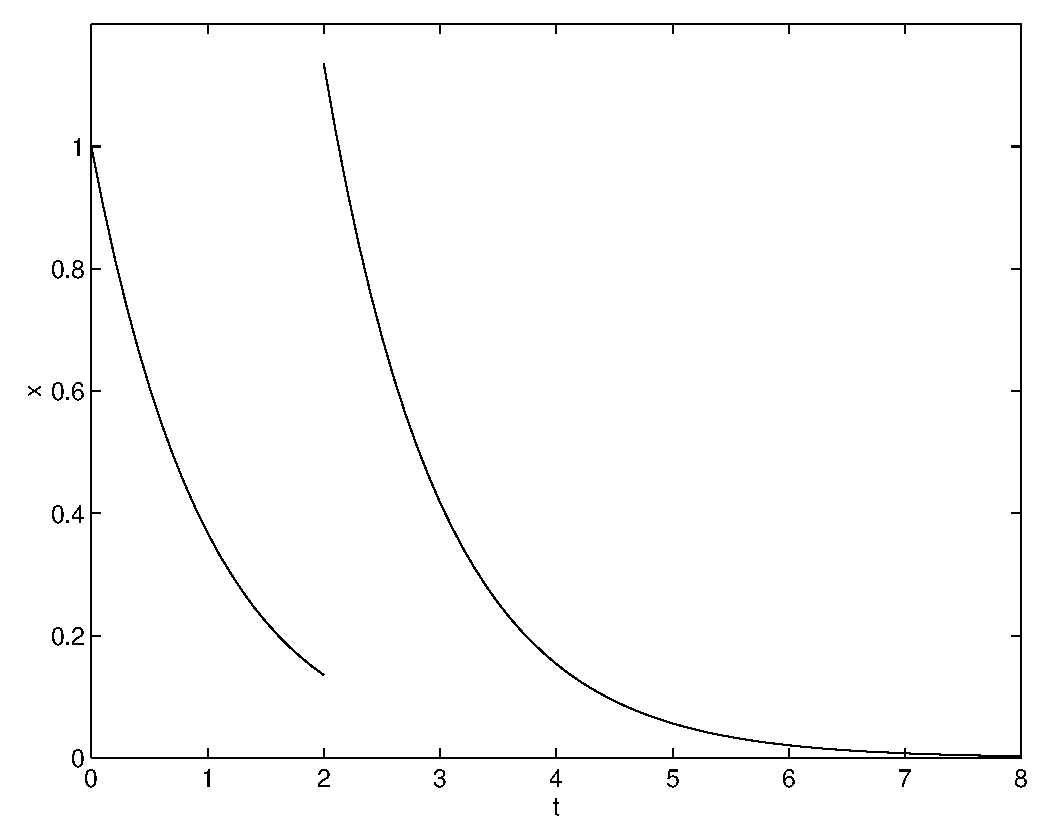
\psfig{file=figures/d1sol.eps,width=2.8in}}
           \caption{The solution of the initial value problem
	   \protect\Ref{eq:delta1}.}
           \label{fig:delta1sol}
\end{figure}


\subsection*{Grand Finale}

We end this section by using Laplace transforms to solve the initial 
value problem:
\begin{equation}  \label{eq:lapendexam}
\begin{array}{rcl}
\ddot x + 4\dot x +5x  & = & \delta_1(t)+2H_3(t) \\
x(0) & = & 0 \\
\dot x(0) & = & 1.
\end{array}
\end{equation}
When solving \Ref{eq:lapendexam} we use most of the techniques that we have 
introduced so far.  

Applying the Laplace transform to both sides of the differential
equation in \Ref{eq:lapendexam} and using the initial conditions leads to
\[
s^2{\cal L}[x] -1 + 4s{\cal L}[x] + 5{\cal L}[x]=
e^{-s} +2\frac{e^{-3s}}{s}.
\]
Solving this equation for the Laplace transform of $x$ yields
\[
{\cal L}[x] = \frac{e^{-s} +2\frac{e^{-3s}}{s}+1}{s^2+4s+5}
= \frac{e^{-s}+1}{s^2+4s+5}+ \frac{2e^{-3s}}{s(s^2+4s+5)}.
\]

To find the inverse Laplace transform\index{Laplace transform!inverse}
of this equation, we need to 
compute the partial fraction expansion of 
\[
\frac{p(s)}{q(s)} = \frac{1}{s(s^2+4s+5)}.
\]
Defining {\tt p=[1]} and {\tt q=[1 4 5 0]} we use the 
command {\tt [c,r] = residue(p,q)}\index{\computer!residue} to obtain 
\begin{verbatim}
c =
  -0.1000 + 0.2000i
  -0.1000 - 0.2000i
   0.2000          
r =
  -2.0000 + 1.0000i
  -2.0000 - 1.0000i
        0          
\end{verbatim}

Hence the roots of $s^2+4s+5$ are $-2\pm i$, and we have
\[
\frac{1}{s(s^2+4s+5)} = \frac{-0.1 + 0.2i}{s-(-2+i)}+
\frac{-0.1-0.2i}{s-(-2-i)}+\frac{0.2}{s}.
\]
We combination the complex conjugate terms by typing
\begin{verbatim}
[num,denom] = realform(c(1),r(1))
\end{verbatim}\index{partial fractions!in \Matlab!{\tt realform}}
and obtain
\begin{verbatim}
num =
    -0.2000   -0.4000
denom =
     -2     1
\end{verbatim}
The partial fractions result is:
\[
\frac{1}{s(s^2+4s+5)} = -\frac{0.2(s+2)+0.4}{(s+2)^2+1}
+\frac{0.2}{s}.
\]

Now we can rewrite ${\cal L}[x]$ as
\begin{eqnarray*}
{\cal L}[x] &=& \frac{e^{-s}}{(s+2)^2+1}+ \frac{1}{(s+2)^2+1}\\
&& +2e^{-3s}\left(-0.2\frac{s+2}{(s+2)^2+1}-0.4\frac{1}{(s+2)^2+1}
+0.2\frac{1}{s}\right).
\end{eqnarray*}
We use Proposition~\ref{prop:eHcLap1}(a) to see that
\begin{eqnarray*}
{\cal L}\inv\left[\frac{1}{(s+2)^2+1}\right]&=&
e^{-2t}\sin(t)\\
{\cal L}^{-1}\left[\frac{s+2}{(s+2)^2+1}\right]&=&
e^{-2t}\cos(t),
\end{eqnarray*}
and Proposition~\ref{prop:eHcLap2}(b) to see that
\begin{eqnarray*}
{\cal L}^{-1}\left[e^{-s}\frac{1}{(s+2)^2+1}\right]&=&
H_1(t)e^{-2(t-1)}\sin(t-1)\\
{\cal L}^{-1}\left[e^{-3s}\frac{s+2}{(s+2)^2+1}\right]&=&
H_3(t)e^{-2(t-3)}\cos(t-3)\\
{\cal L}^{-1}\left[e^{-3s}\frac{1}{(s+2)^2+1}\right]&=&
H_3(t)e^{-2(t-3)}\sin(t-3).
\end{eqnarray*}
Now we can write down the solution $x(t)$ as
\begin{eqnarray*}
x(t) &=& H_1(t)e^{-2(t-1)}\sin(t-1)+e^{-2t}\sin(t)\\
&&-0.4 H_3(t)e^{-2(t-3)}\cos(t-3) -0.8 H_3(t)e^{-2(t-3)}\sin(t-3)
+0.4 H_3(t)\\
&=& H_1(t)e^{-2(t-1)}\sin(t-1)+e^{-2t}\sin(t)\\
&& -0.4 H_3(t)e^{-2(t-3)}(\cos(t-3)+2\sin(t-3))+0.4 H_3(t).
\end{eqnarray*}
The solution is shown in Figure~\ref{fig:lapallsol}.
The two changes in the behavior of the solution occurring at 
$t=1$ and at $t=3$ are readily observed.  
\begin{figure}[htb]
           \centerline{%
           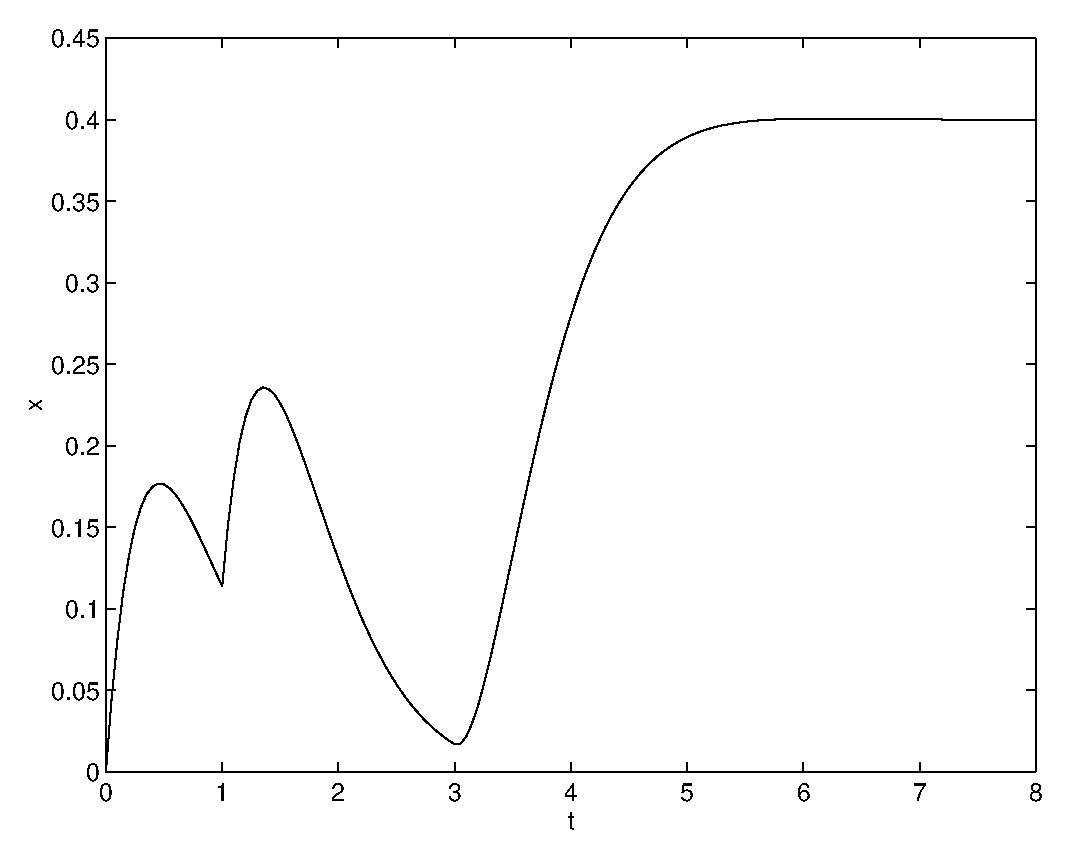
\psfig{file=figures/dallsol.eps,width=3.2in}}
           \caption{The solution of the initial value problem
           \protect\Ref{eq:lapendexam}.}
           \label{fig:lapallsol}
\end{figure}

Note that the solution to \Ref{eq:lapendexam} tends asymptotically to 
$x=0.4$  for large $t$.  This behavior can be explained as follows.  For large 
$t$, equation \Ref{eq:lapendexam} becomes
\[
\ddot x + 4\dot x +5x = 2.
\]
The only equilibrium (or time independent solution) to this equation is
$x(t)=0.4$, and each solution of \Ref{eq:lapendexam} tends to that equilibrium 
for large $t$.


\EXER

\TEXER

\begin{exercise}  \label{Ex:cont}
Consider the function
\[
z(t) = H_1(t)(1-\cos(2(t-1))) = \left\{
\begin{array}{cl} 0 & t \leq 1 \\ 1-\cos(2(t-1)) & t > 1. \end{array}\right.
\]
Show that $z(t)$ is continuous at $t=1$ by verifying that 
\[
\lim_{t\to 1^+}z(t) = \lim_{t\to 1^-}z(t).
\]
Show that $z(t)$ is differentiable and that $\dot{z}(1)=0$ by verifying that 
\[
\lim_{h\to 0^+} \frac{z(1+h)-z(1)}{h} = 0 = 
\lim_{h\to 0^-} \frac{z(1+h)-z(1)}{h}
\]
\end{exercise}

\begin{exercise} \label{c13.4.2}
Reconfirm that the solution of the initial value problem
\[
\ddot x + 4 x=H_1(t),\quad x(0)=1,\quad \dot x(0)=0
\]
is given by
\[
x(t)=\frac{1}{4}H_1(t)(1-\cos(2(t-1))) + \cos(2t).
\]
Use the methods of Chapter \ref{C:LDE} and proceed as follows:
\begin{itemize}
\item[(a)] Find the solution $x_1(t)$ of the initial value problem
\[
\ddot x + 4 x=0,\quad x(0)=1,\quad \dot x(0)=0
\]
on the time interval $t\in[0,1]$.
\item[(b)] Find the general solution $x_2(t)$ of the second order
differential equation $\ddot x + 4 x=1$.
\item[(c)] Adjust the parameters in $x_2(t)$ such that the function
\[
x(t)=\left\{ \begin{array}{l} x_1(t)\quad t\in[0,1]\\
x_2(t) \quad t>1 \end{array}\right.
\]
is differentiable at $t=1$.
\end{itemize}
\end{exercise}



\CEXER



\begin{exercise} \label{c13.4.5}
Use the \Matlab command {\tt ode45} to compute the solution of the grand 
finale initial value problem \Ref{eq:lapendexam}.  
More precisely, write \Ref{eq:lapendexam} as a nonautonomous first order 
system of ODEs by setting $y=\dot{x}$ and obtaining
\begin{equation*}
\begin{array}{rcl}
\dot{x} & = & y \\
\dot{y} & = & -5x-4y+\delta_1(t)+2H_3(t).
\end{array}
\end{equation*}

There is a numerical difficulty when attempting to compute delta functions. 
A standard way around this difficulty is to approximate the Dirac delta 
function $\delta_1(t)$ using \Ref{eq:deltah} with $h=0.01$.  We use the 
\Matlab m-file {\tt f16\_4\_5.m} for the numerical computations:
\begin{verbatim}
function y = f16_4_5(t,x)
   h = 0.01;
y(1) = x(2);
y(2) = -4*x(2)-5*x(1);
if (abs(t-(1-h/2)) <= h/2)
        y(2) = y(2) + 1/h;
end
if (t >= 3)
        y(2) = y(2) + 2;
end
y = [y(1) y(2)]';
\end{verbatim}\index{\computer!abs}

Using {\tt ode45}\index{\computer!ode45} compute the solution on the 
time interval $[0,8]$ using the command
\begin{verbatim}
[t,x] = ode45('f16_4_5',[0 8],[0,1]); 
\end{verbatim}
Plot the first component of {\tt x} by typing {\tt plot(t,x(:,1))} and observe 
the difference between the numerically computed solution and the exact 
solution, whose graph is plotted in Figure~\ref{fig:lapallsol}.

Next, set the relative error tolerance {\tt 1e-8} using the command
\begin{verbatim}
options = odeset('RelTol',1e-8);
\end{verbatim}
and compute the solution using the command
\begin{verbatim}
[t,x] = ode45('f16_4_5',[0 8],[0,1],options); 
\end{verbatim}
Compare the results of this numerical integration with the theoretically exact 
result in Figure~\ref{fig:lapallsol}.  Try to explain why the results differ 
for different tolerances.
\end{exercise}


\section{RLC Circuits}  \label{S:SOFE}
\index{RLC circuit}\index{electrical circuit}

RLC circuits provide an excellent example of a physical system that is well
modeled by a second order linear differential equation that is periodically 
forced by a discontinuous function.  Consider the electrical circuit shown in 
Figure~\ref{fig:rcl}.  The circuit consists of a resistor\index{resistor} with
resistance $R$, a coil\index{coil} with inductance $L$, a 
capacitor\index{capacitor} with 
capacitance $C$, and a voltage source\index{voltage source} producing a time 
dependent voltage $V(t)$.    
\begin{figure}[htb]
           \centerline{%
           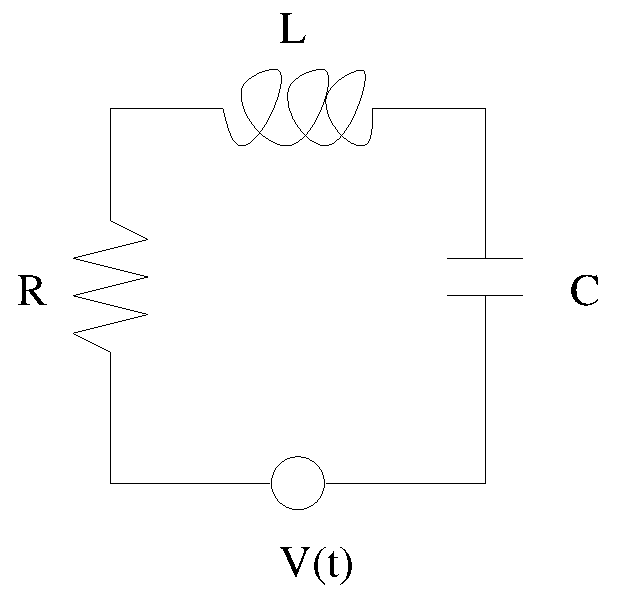
\psfig{file=figures/rcl.eps,width=2.0in}}
           \caption{An RLC circuit with resistance $R$, inductance $L$,
	   capacitance $C$, and a voltage source $V(t)$.}
           \label{fig:rcl}
\end{figure}

We describe the behavior of the circuit by the voltage drop $x(t)$ at the 
capacitor.  Kirchhoff's Laws\index{Kirchhoff's laws} 
for electric circuits show that $x(t)$ satisfies 
the second order differential equation
\begin{equation}  \label{e:eleccirc}
\frac{1}{CL}V(t) = \frac{d^2x}{dt^2}(t) + \frac{R}{L}\frac{dx}{dt}(t) + 
\frac{1}{CL}x(t),
\end{equation}
as we now explain.   {\em Kirchhoff's Voltage 
Law\/}\index{Kirchhoff's laws} states that at each
instant of time the voltage $V(t)$ produced at the source is
equal to the sum of the voltage drops at the three elements of
the circuit.  So, if we denote the voltage drops at the coil\index{coil}
by $V_{coil}$ and at the resistor\index{resistor} by $V_{resistor}$, then 
we have 
\begin{equation}  \label{e:kirchhoff}
V(t) = V_{coil}(t) + V_{resistor}(t) + x(t),
\end{equation}
recalling that $x(t)$ is the voltage drop at the capacitor\index{capacitor}.

Let $I(t)$ be the current through the system.  Then 
\begin{itemize}
\item[(a)]  The voltage drop in a capacitor is proportional to the charge 
difference $Q_{capacitor}$ between the two plates:
\[
x(t) = \frac{1}{C}Q_{capacitor},
\]
where $C$ is the {\em capacitance\/} measured in farads.  The charge 
difference itself is related to the current by 
\[
I = \frac{dQ_{capacitor}}{dt} = C\frac{dx}{dt}.
\]
\item[(b)]  The voltage drop at a resistor is proportional to the current:	
\[
V_{resistor} = RI = RC\frac{dx}{dt},
\]
where $R$ is the {\em resistance\/} measured in ohms.
\item[(c)]  The voltage drop in a coil\index{coil} is given by 
{\em Faraday's Law}\index{Faraday's law}; 
the drop is proportional to the rate of change of the current\index{current}:
\[
V_{coil} = L\frac{dI}{dt} = LC\frac{d^2x}{dt^2},
\]
where $L$ is the inductance of the coil measured in henrys.
\end{itemize}

Combining (a,b,c) with \Ref{e:kirchhoff}, we obtain the differential equation:
\[
V(t) = LC\ddot{x} + RC\dot{x} +  x.
\]
After dividing by $LC$, we obtain the second order equation \Ref{e:eleccirc};
and, on setting 
\[
a = \frac{R}{L}, \quad b = \frac{1}{CL}, \AND g(t) = \frac{1}{CL}V(t),
\] 
we have an initial value problem in the form \Ref{e:2ndforced}.

A typical input at the voltage source\index{voltage source} 
(associated to alternating current) is 
a $2T$-periodic square wave with amplitude $A>0$ defined by periodicity and
\[
V(t) = \left\{\begin{array}{rl} A & 0<t\leq T\\
			       -A & T<t\leq 2T.
	\end{array}\right.
\]
See Figure~\ref{fig:sq}.  We will see how to use Laplace transforms to solve 
second order equations with a discontinuous forcing\index{forcing!discontinuous} 
of this type.  Indeed,
it is the possibility of using Laplace transforms to solve linear equations 
with piecewise smooth forcing terms\index{forcing!piecewise smooth} that is 
the main strength of Laplace
transforms.

\begin{figure}[htb]
           \centerline{%
           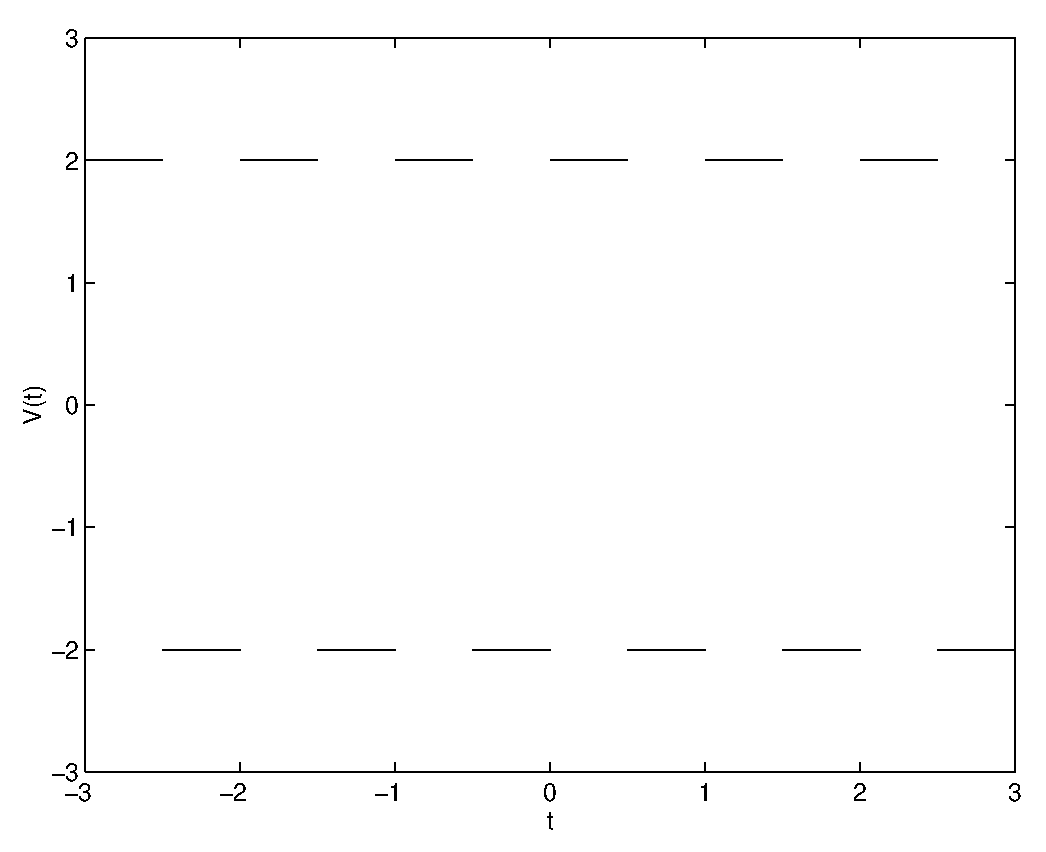
\psfig{file=figures/sq.eps,width=3.0in}}
           \caption{A 1-periodic square wave $V(t)$ of amplitude $A=2$.}
           \label{fig:sq}
\end{figure}


\subsection*{Piecewise Smooth Periodic Forcing}
\index{forcing!piecewise smooth!periodic}

We now show how Laplace transforms can be used to solve second order
equations with periodic discontinuous forcing.  As an example we consider
the equation \Ref{eq:ivH1} where the external force $g(t)$ is
given by
\begin{equation}
g(t) =  
\left\{\begin{array}{cl} 1 & \mbox{for $t \in [2k,2k+1]$} \\ 
		0 & \mbox{for $t \in [2k+1,2k+2]$} \end{array} \right.
(k=0,1,2,\ldots).
\end{equation}
We begin by computing the Laplace transform of $g(t)$. Using the 
definition we obtain
\begin{eqnarray*}
{\cal L}[g] & = & \int_0^\infty e^{-st} g(t)\, dt\\
&=& \sum_{k=0}^\infty \int_k^{k+1} e^{-st} g(t)\, dt\\
&=& \sum_{k=0}^\infty \int_{2k}^{2k+1} e^{-st}\, dt,
\end{eqnarray*}
since $g(t)$ vanishes for $t \in [2k+1,2k+2]$. Performing the
integrations leads to
\begin{eqnarray*}
{\cal L}[g] & = & \frac{1}{s}\sum_{k=0}^\infty \left(e^{-2sk}-e^{-s(2k+1)}\right)\\
&=& \frac{1}{s}\sum_{k=0}^\infty (1-e^{-s})e^{-2sk}\\
&=& \frac{1}{s} (1-e^{-s}) \frac{1}{1-e^{-2s}}\\
&=& \frac{1}{s(1+e^{-s})}.
\end{eqnarray*}
Hence an application of the Laplace transform to the differential equation 
\Ref{eq:ivH1} gives
\[
s^2{\cal L}[x]-s + 4{\cal L}[x] = {\cal L}[g] = \frac{1}{s(1+e^{-s})},
\]
and solving this for ${\cal L}[x]$ leads to
\[
{\cal L}[x] = \frac{1}{s(s^2 +4)(1+e^{-s})} + \frac{s}{s^2 +4}.
\]
It remains to compute the inverse Laplace transform\index{Laplace transform!inverse} 
of the first term.  For this
we observe that for real numbers $x$ with $|x|<1$ the following identity holds:
\[
\frac{1}{1+x} = 1-x+x^2-x^3+x^4-\cdots = \sum_{k=0}^\infty (-1)^k x^k.
\]
Hence, for positive $s$,
\[
\frac{1}{1+e^{-s}} = \sum_{k=0}^\infty (-1)^k e^{-sk},
\]
and it follows that
\begin{eqnarray*}
{\cal L}[x] &=&\frac{1}{s(s^2 +4)}\sum_{k=0}^\infty (-1)^k e^{-sk} + \frac{s}{s^2 +4}\\
&=& \frac{1}{4}\left(\frac{1}{s}-\frac{s}{s^2+4}\right)
    \sum_{k=0}^\infty (-1)^k e^{-sk} + \frac{s}{s^2 +4}\\
&=& \frac{1}{4}\left(\frac{1}{s}+\frac{3s}{s^2+4}+
   \left(\frac{1}{s}-\frac{s}{s^2+4}\right) \sum_{k=1}^\infty (-1)^k e^{-sk}\right)\\
&=& \frac{1}{4}\left(\frac{1}{s}+\frac{3s}{s^2+4}+
   \sum_{k=1}^\infty (-1)^k \frac{e^{-sk}}{s}-
   \sum_{k=1}^\infty (-1)^k \frac{e^{-sk}s}{s^2+4}\right).
\end{eqnarray*} 
Now we have derived an expression for ${\cal L}[x]$ in which we can compute the
inverse Laplace transform for each of the individual summands.  Using 
Table~\ref{tab:Laplist} and Proposition~\ref{prop:eHcLap2} we obtain
\begin{eqnarray*}
x(t)&=&\frac{1}{4}\left(1+3\cos(2t)+\sum_{k=1}^\infty (-1)^k H_k(t)
       -\sum_{k=1}^\infty (-1)^k H_k(t)\cos(2(t-k))\right)\\
&=&\frac{1}{4}\left(1+3\cos(2t)+\sum_{k=1}^\infty (-1)^k H_k(t)(1-\cos(2(t-k)))\right)\\
&=&\frac{1}{4}\left(1+3\cos(2t)+2\sum_{k=1}^\infty (-1)^k H_k(t)\sin^2(t-k))\right).
\end{eqnarray*}
In Figure~\ref{fig:lapperi} we show the solution for $t\in [0,20]$.  Observe 
that this solution is certainly not periodic in time.  Indeed, since the 
internal frequency\index{frequency!internal} of equation \Ref{eq:ivH1} is 
$1/\pi$ and the frequency of the external periodic forcing is $1/2$ we expect 
to obtain a quasiperiodic motion\index{motion!quasiperiodic}.
\begin{figure}[htb]
           \centerline{%
           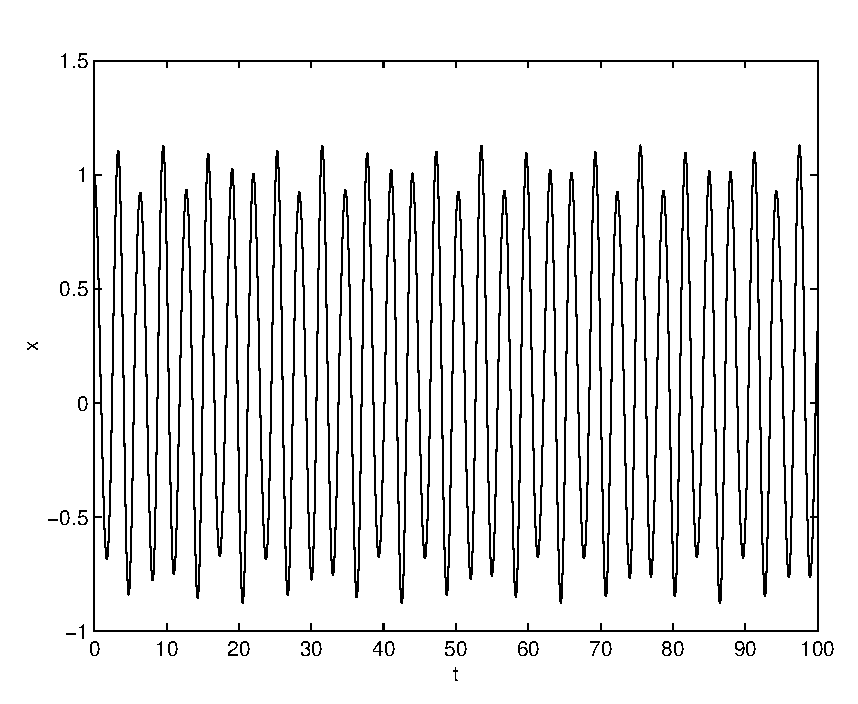
\psfig{file=figures/lapperi.eps,width=3.5in}}
           \caption{The solution of the initial value problem
	   \protect\Ref{eq:ivH1} where the external force is
   	   given by a periodic discontinuous function.}
           \label{fig:lapperi}
\end{figure}






\end{document}
